\documentclass[a4paper,final]{article}
\usepackage[14pt]{extsizes}
\usepackage[T2A]{fontenc}
\usepackage[utf8]{inputenc}
\usepackage[russian]{babel}
\usepackage{amsmath}
\usepackage[left=20mm, top=20mm, right=20mm, bottom=20mm, footskip=10mm]{geometry}
\usepackage{ragged2e}
\usepackage{setspace}
\usepackage{alltt}
\usepackage{wrapfig}
\usepackage{moreverb} %листинги
\usepackage{indentfirst} % для абзацного отступа
\renewcommand\verbatimtabsize{4\relax}
\renewcommand\listingoffset{0.2em} %отступ от номеров строк
\renewcommand{\arraystretch}{1.4} % высота строки
\usepackage[font=small, singlelinecheck=false, justification=raggedleft, format=plain, labelsep=period]{caption} %заголовок таблицы
\usepackage{listings}
\usepackage{xcolor} % цвета
\usepackage{hyperref}% для гиперссылок
\usepackage{enumitem} %для перечислений
\usepackage{nccmath}
\usepackage{tikz}
\usepackage{wrapfig}
\usepackage{listings}
\usepackage{float}
\usepackage{shadow}
\usepackage{longtable}
\usepackage{multirow}
\usepackage{makecell}
\usepackage{longtable}
\usepackage{tabularx}

\hypersetup{colorlinks,
  allcolors=[RGB]{000 000 000}} %гиперссылки

\textheight=24cm
\textwidth=16cm
\oddsidemargin=0pt
\topmargin=-1.5cm
\parindent=24pt % отступ абзаца по горизонтали
\parskip=5pt % отступ абзаца по вертикали
\tolerance=2000 % терпимость
\flushbottom % выравнивание высоты
\addto\captionsrussian{\def\refname{Список использованной литературы}}
\usepackage{xcolor}

%New colors defined below
\definecolor{codegreen}{rgb}{0,0.6,0}
\definecolor{codegray}{rgb}{0.5,0.5,0.5}
\definecolor{codepurple}{rgb}{0.58,0,0.82}
\definecolor{backcolour}{rgb}{0.95,0.95,0.92}


\definecolor{apricot}{HTML}{FFF0DA}
\definecolor{mygreen}{rgb}{0,0.6,0}
\definecolor{string}{HTML}{B40000} % цвет строк в коде
\definecolor{comment}{HTML}{008000} % цвет комментариев в коде
\definecolor{keyword}{HTML}{1A00FF} % цвет ключевых слов в коде
\definecolor{morecomment}{HTML}{8000FF} % цвет include и других элементов в коде
\definecolor{captiontext}{HTML}{FFFFFF} % цвет текста заголовка в коде
\definecolor{captionbk}{HTML}{999999} % цвет фона заголовка в коде
\definecolor{bk}{HTML}{FFFFFF} % цвет фона в коде
\definecolor{frame}{HTML}{999999} % цвет рамки в коде
\definecolor{brackets}{HTML}{B40000} % цвет скобок в коде

\setlist[enumerate,itemize]{leftmargin=1.2cm}

% подгружаемые языки — подробнее в документации listings
\lstloadlanguages{C++}

\newcommand{\doublecline}[1]{\noalign{\vskip-0.5\arrayrulewidth}\cline{#1}\noalign{\vskip-0.5\arrayrulewidth}\cline{#1}}

\begin{document}
\lstset{
  language=C++, % Язык кода по умолчанию
  morekeywords={*,...}, % если хотите добавить ключевые слова, то добавляйте
  % Цвета
  keywordstyle=\color{keyword}\ttfamily\bfseries,
  %stringstyle=\color{string}\ttfamily,
  stringstyle=\ttfamily\color{red!50!brown},
  commentstyle=\color{comment}\ttfamily,
  morecomment=[l][\color{morecomment}]{\#},
  % Настройки отображения
  breaklines=true, % Перенос длинных строк
  basicstyle=\ttfamily\footnotesize, % Шрифт для отображения кода
  backgroundcolor=\color{bk}, % Цвет фона кода
  frame=lrb,xleftmargin=\fboxsep,xrightmargin=-\fboxsep, % Рамка, подогнанная к заголовку
  rulecolor=\color{frame}, % Цвет рамки
  tabsize=3, % Размер табуляции в пробелах
  % Настройка отображения номеров строк. Если не нужно, то удалите весь блок
  numbers=left, % Слева отображаются номера строк
  stepnumber=1, % Каждую строку нумеровать
  numbersep=5pt, % Отступ от кода
  numberstyle=\small\color{black}, % Стиль написания номеров строк
  % Для отображения русского языка
  extendedchars=true,
  literate={Ö}{ {\"O} }1
  {~}{ {\textasciitilde} }1
  {а}{ {\selectfont\char224} }1
  {б}{ {\selectfont\char225} }1
  {в}{ {\selectfont\char226} }1
  {г}{ {\selectfont\char227} }1
  {д}{ {\selectfont\char228} }1
  {е}{ {\selectfont\char229} }1
  {ё}{ {\"e} }1
  {ж}{ {\selectfont\char230} }1
  {з}{ {\selectfont\char231} }1
  {и}{ {\selectfont\char232} }1
  {й}{ {\selectfont\char233} }1
  {к}{ {\selectfont\char234} }1
  {л}{ {\selectfont\char235} }1
  {м}{ {\selectfont\char236} }1
  {н}{ {\selectfont\char237} }1
  {о}{ {\selectfont\char238} }1
  {п}{ {\selectfont\char239} }1
  {р}{ {\selectfont\char240} }1
  {с}{ {\selectfont\char241} }1
  {т}{ {\selectfont\char242} }1
  {у}{ {\selectfont\char243} }1
  {ф}{ {\selectfont\char244} }1
  {х}{ {\selectfont\char245} }1
  {ц}{ {\selectfont\char246} }1
  {ч}{ {\selectfont\char247} }1
  {ш}{ {\selectfont\char248} }1
  {щ}{ {\selectfont\char249} }1
  {ъ}{ {\selectfont\char250} }1
  {ы}{ {\selectfont\char251} }1
  {ь}{ {\selectfont\char252} }1
  {э}{ {\selectfont\char253} }1
  {ю}{ {\selectfont\char254} }1
  {я}{ {\selectfont\char255} }1
  {А}{ {\selectfont\char192} }1
  {Б}{ {\selectfont\char193} }1
  {В}{ {\selectfont\char194} }1
  {Г}{ {\selectfont\char195} }1
  {Д}{ {\selectfont\char196} }1
  {Е}{ {\selectfont\char197} }1
  {Ё}{ {\"E} }1
  {Ж}{ {\selectfont\char198} }1
  {З}{ {\selectfont\char199} }1
  {И}{ {\selectfont\char200} }1
  {Й}{ {\selectfont\char201} }1
  {К}{ {\selectfont\char202} }1
  {Л}{ {\selectfont\char203} }1
  {М}{ {\selectfont\char204} }1
  {Н}{ {\selectfont\char205} }1
  {О}{ {\selectfont\char206} }1
  {П}{ {\selectfont\char207} }1
  {Р}{ {\selectfont\char208} }1
  {С}{ {\selectfont\char209} }1
  {Т}{ {\selectfont\char210} }1
  {У}{ {\selectfont\char211} }1
  {Ф}{ {\selectfont\char212} }1
  {Х}{ {\selectfont\char213} }1
  {Ц}{ {\selectfont\char214} }1
  {Ч}{ {\selectfont\char215} }1
  {Ш}{ {\selectfont\char216} }1
  {Щ}{ {\selectfont\char217} }1
  {Ъ}{ {\selectfont\char218} }1
  {Ы}{ {\selectfont\char219} }1
  {Ь}{ {\selectfont\char220} }1
  {Э}{ {\selectfont\char221} }1
  {Ю}{ {\selectfont\char222} }1
  {Я}{ {\selectfont\char223} }1
  {\{}{ { {\color{brackets}\{} } }1 % Цвет скобок {
  {\} }{ { {\color{brackets}\} } } }1 % Цвет скобок }
}
\thispagestyle{empty}
\begin{center}
\hfill \break
\hfill \break
\normalsize{МИНИСТЕРСТВО НАУКИ И ВЫСШЕГО ОБРАЗОВАНИЯ РОССИЙСКОЙ ФЕДЕРАЦИИ\\
 федеральное государственное автономное образовательное учреждение высшего образования «Санкт-Петербургский политехнический университет Петра Великого»\\[10pt]}
\normalsize{Институт компьютерных наук и кибербезопасности}\\[10pt] 
\normalsize{Высшая школа технологий искусственного интеллекта}\\[10pt] 
\normalsize{Направление: 02.03.01 <<Математика и компьютерные науки>>}\\
\vspace{75pt}
{\large Математическая логика и теория формальных языков\\
Отчёт о выполнении лабораторной работы №1 \\
<<Лексический анализатор>>\\[1em]
Вариант 35}
\end{center}
 \vspace{80pt}
\small{ 
\begin{tabular}{lrrl}
\!\!\!Студент, & \hspace{2cm} & & \\
\!\!\!группа 5130201/30102 & \hspace{2cm} & \underline{\hspace{3cm}} & Путята М. А.  \\\\
\!\!\!Преподаватель & \hspace{2cm} & \underline{\hspace{3cm}} &  Востров А. В. \\\\
&&\hspace{5cm}
\end{tabular}
\begin{flushright}
<<\underline{\hspace{1cm}}>>\underline{\hspace{2.5cm}} 2026 г.
\end{flushright}
}

\hfill \break
\begin{center} \small{Санкт-Петербург, 2026} \end{center}


\newpage
\tableofcontents
\newpage

\section*{Введение}
\addcontentsline{toc}{section}{Введение}
Компиляция программы -- это процесс трансляции исходного кода программы из одного языка в другой (обычно в более низкоуровневый, например в машинный код). Компиляция состоит из следующих основных этапов:
\begin{enumerate}
    \item \textbf{Препроцессинг}. Разрешение зависимостей и обработка макросов (директивы препроцессора).
    \item \textbf{Лексический анализ}. Выделение лексем в исходном коде программы и получение представления исходной программы как последовательности лексических единиц.
    \item \textbf{Синтаксический анализ}. Проверка грамматики языка и создание синтаксического дерева, представляющего структуру программы.
    \item \textbf{Семантический анализ}. Проверка смысловой корректности в контексте правил языка.
    \item \textbf{Генерация кода}. Преобразование созданного в предыдущих этапах представления программы в программу, написанную на другом языке. 
\end{enumerate}

Целью данной работы является разработка программы, выполняющей лексический анализ входного текста в соответствии с заданными требованиями и порождающей таблицу лексем с указанием их типов и значений. Создаваемая программа во время работы должна:
\begin{itemize}
    \item выделять во входном тексте лексемы;
    \item определять типы выделяемых лексем;
    \item проверять длину идентификаторов и строковых констант, ограниченную 15 символами.
    \item допускать комментарии неограниченной длины;
    \item выводить сообщения об ошибках, которые могут быть обнаружены на этапе лексического анализа программы.
\end{itemize}

\textbf{Вариант 35}. Входной язык содержит только латиницу, арифметические выражения, разделённые символом | (вертикальная полоса). Арифметические выражения состоят из идентификаторов, шестнадцатеричных вещественных чисел, знаков операций +, -, *, / и круглых скобок. Шестнадцатеричными числами считать последовательность цифр и символов a, b, c, d, e, f, начинающуюся с <<0x>> (например, 0x89.ab1б 0x45a.0c, 0x0.0af).

\newpage
\section{Математическое описание}
\subsection{Транслятор}
\begin{figure}[H]
    \centering
    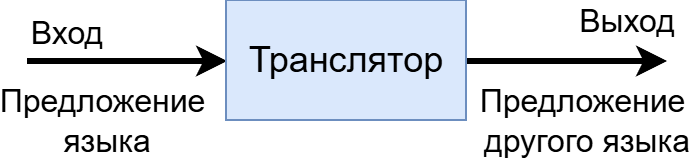
\includegraphics[width=0.5\linewidth]{Транслятор.png}
    \caption{\centeringТранслятор}
\end{figure}
Транслятор - алгоритм преобразования предложения исходного языка в некоторый выход. Если входной текст является алгоритмическим, то входной текст называют входной программой.

Если задачей транслятора является преобразование в язык низкого уровня, то он называется компилятором, а если выполнение операторов исходного кода -- интерпретатором

Процесс синтаксически-ориентированной трансляции состоит из двух этапов:
\begin{itemize}
    \item Распознавание исходного языка. Построение структуры входного текста на основе порождающей грамматики входного языка.
    \item Генерация выхода. Использование полученной на предыдущем этапе структуры для создание выхода, удовлетворяющему семантике исходного текста.
\end{itemize}

\subsection{Лексический анализатор}

Лексический анализатор проводит лексический анализ (первый этап трансляции), выделяя лексемы входного языка -- минимальные единицы языка, которые имеют смысл. В естественном языке лексемами являются слова, а в языке программирования -- идентификаторы, служебные символы, константы, операторы и т.д..

\paragraph{Предназначение\\[1em]}

Лексический анализ предназначен для определения:
\begin{itemize}
    \item лексем -- подстрок символов, соответствующих распознанным классам лексем.
    \item классов обнаруживаемых лексем -- общее название для категории элементов, обладающих общими свойствами: идентификатор, вещественная константа, строковая константа, операторы и т.д..
\end{itemize}

\paragraph{Классификация символов входного текста\\[1em]}

На вход лексическому анализатору подаются символы, сгруппированные транслитератором по определённым категориям. Наиболее типичные группы символов:
\begin{itemize}
    \item \textbf{буква} -- множество букв, из 1 и более алфавитов.
    \item \textbf{цифра} -- множество символов, относящихся к цифрам, чаще всего от 0 до 9 (для шестнадцатеричной системы счисления от 0 до f).
    \item \textbf{разделитель} -- пробел, перевод строки, возврат каретки.
    \item \textbf{игнорируемый} -- символы, которые могут присутствовать во входнмо потоке, но игнорируемые анализатором.
    \item \textbf{запрещённый} -- символы, не входящие в алфавит языка.
    \item \textbf{прочие} -- символы не принадлежащие к предыдущим категориям.
\end{itemize}

\paragraph{Формальная модель\\[1em]}
Лексический анализатор реализуется с помощью конечного автомата, преобразующего входную цепочку символов в последовательность пар <Тип лексемы, Значение>.

Если заданы:
\begin{itemize}
    \item $\displaystyle \Sigma$ = \{\textbackslash t, \textbackslash n, ''\_'', (, ), *, +, -, /, ., :, =, |\} $\cup$ \{0, \dots, 9]\} $\cup$ \{A, \dots, Z\} $\cup$ \{ a, \dots, z \} -- входной алфавит;
    \item $\displaystyle T$ = \{ id, arithmetic, assign, left\_bracket, right\_bracket, const, separator \} -- множество типов лексем, где
    \begin{itemize}
        \item id -- идентификатор;
        \item assign -- знак присваивания <<:=>>
        \item arithmetic -- арифметический оператор (<<+>>, <<->>, <<*>>, <</>>);
        \item left\_bracket, right\_bracket -- левая и правая круглые скобки соответственно;
        \item const -- вещественная константа, записанная в шестнадцатеричной системе счисления (например 0xa65f);
        \item separator -- разделитель <<|>>;
    \end{itemize}
    \item $D$ = \{ :=, +, -, *, /, (, ), | \} $\cup ~D_{id} \cup D_{const}$ -- множество допустимых значений лексем, где
    \begin{itemize}
        \item $D_{id} = \left\{s \in \Sigma_{id}^+~~ \middle|~~\begin{array}{l}
            |s| \in [1, 15], \\
            s[0] \in \{A, \dots, Z\} \cup \{ a, \dots, z \}, \\
            \forall i \in [1, 14]: s[i] \in \Sigma_{id}
        \end{array}
        \right\}$,\\[1em]
        $\Sigma_{id} = \{A, \dots, Z\} \cup \{ a, \dots, z \} \cup \{ 0, \dots, 9 \}$
        \item $D_{const} = \left\{s \in \Sigma_{const}^+~~ \middle|~~\begin{array}{l}
            |s| \in [3, 15], \\
            (s[0] = \text{''0''}) \wedge (s[1] = \text{''x''}) \wedge (s[~|s| - 1~] \neq ~\text{''.''})\\
            |\{ i \in [3, 14] ~|~ s[i] = \text{''.''}\}| \leq 1,\\
            \forall i \in [2, 14]: s[i] \in \Sigma_{const} \setminus \{ \text{''x''} \}
        \end{array}
        \right\}$\\[1em]
        $\Sigma_{const} = \{\text{''x''}\} \cup \{ a, \dots, z \} \cup \{ 0, \dots, 9 \}$
    \end{itemize}
\end{itemize}
То лексический анализатор будет реализовывать отображение $\displaystyle \Sigma^* \longrightarrow (T \times D)^*$, где
\begin{itemize}
    \item $\displaystyle \Sigma^*$ -- замыкание алфавита входного языка;
    \item $(T \times D)^*$ -- множество пар <Тип лексемы, Значение>.
\end{itemize}

\paragraph{Синтаксические диаграммы\\[1em]}
Для представления поведения конечного автомата (в данном случае лексического анализатора) можно использовать синтаксическую диаграмму, получаемую с помощью преобразования КА. Далее на рисунке 1 представлена синтаксическая диаграмма для лексического анализатора, разрабатываемого в данной работе.
\begin{figure}[H]
    \centering
    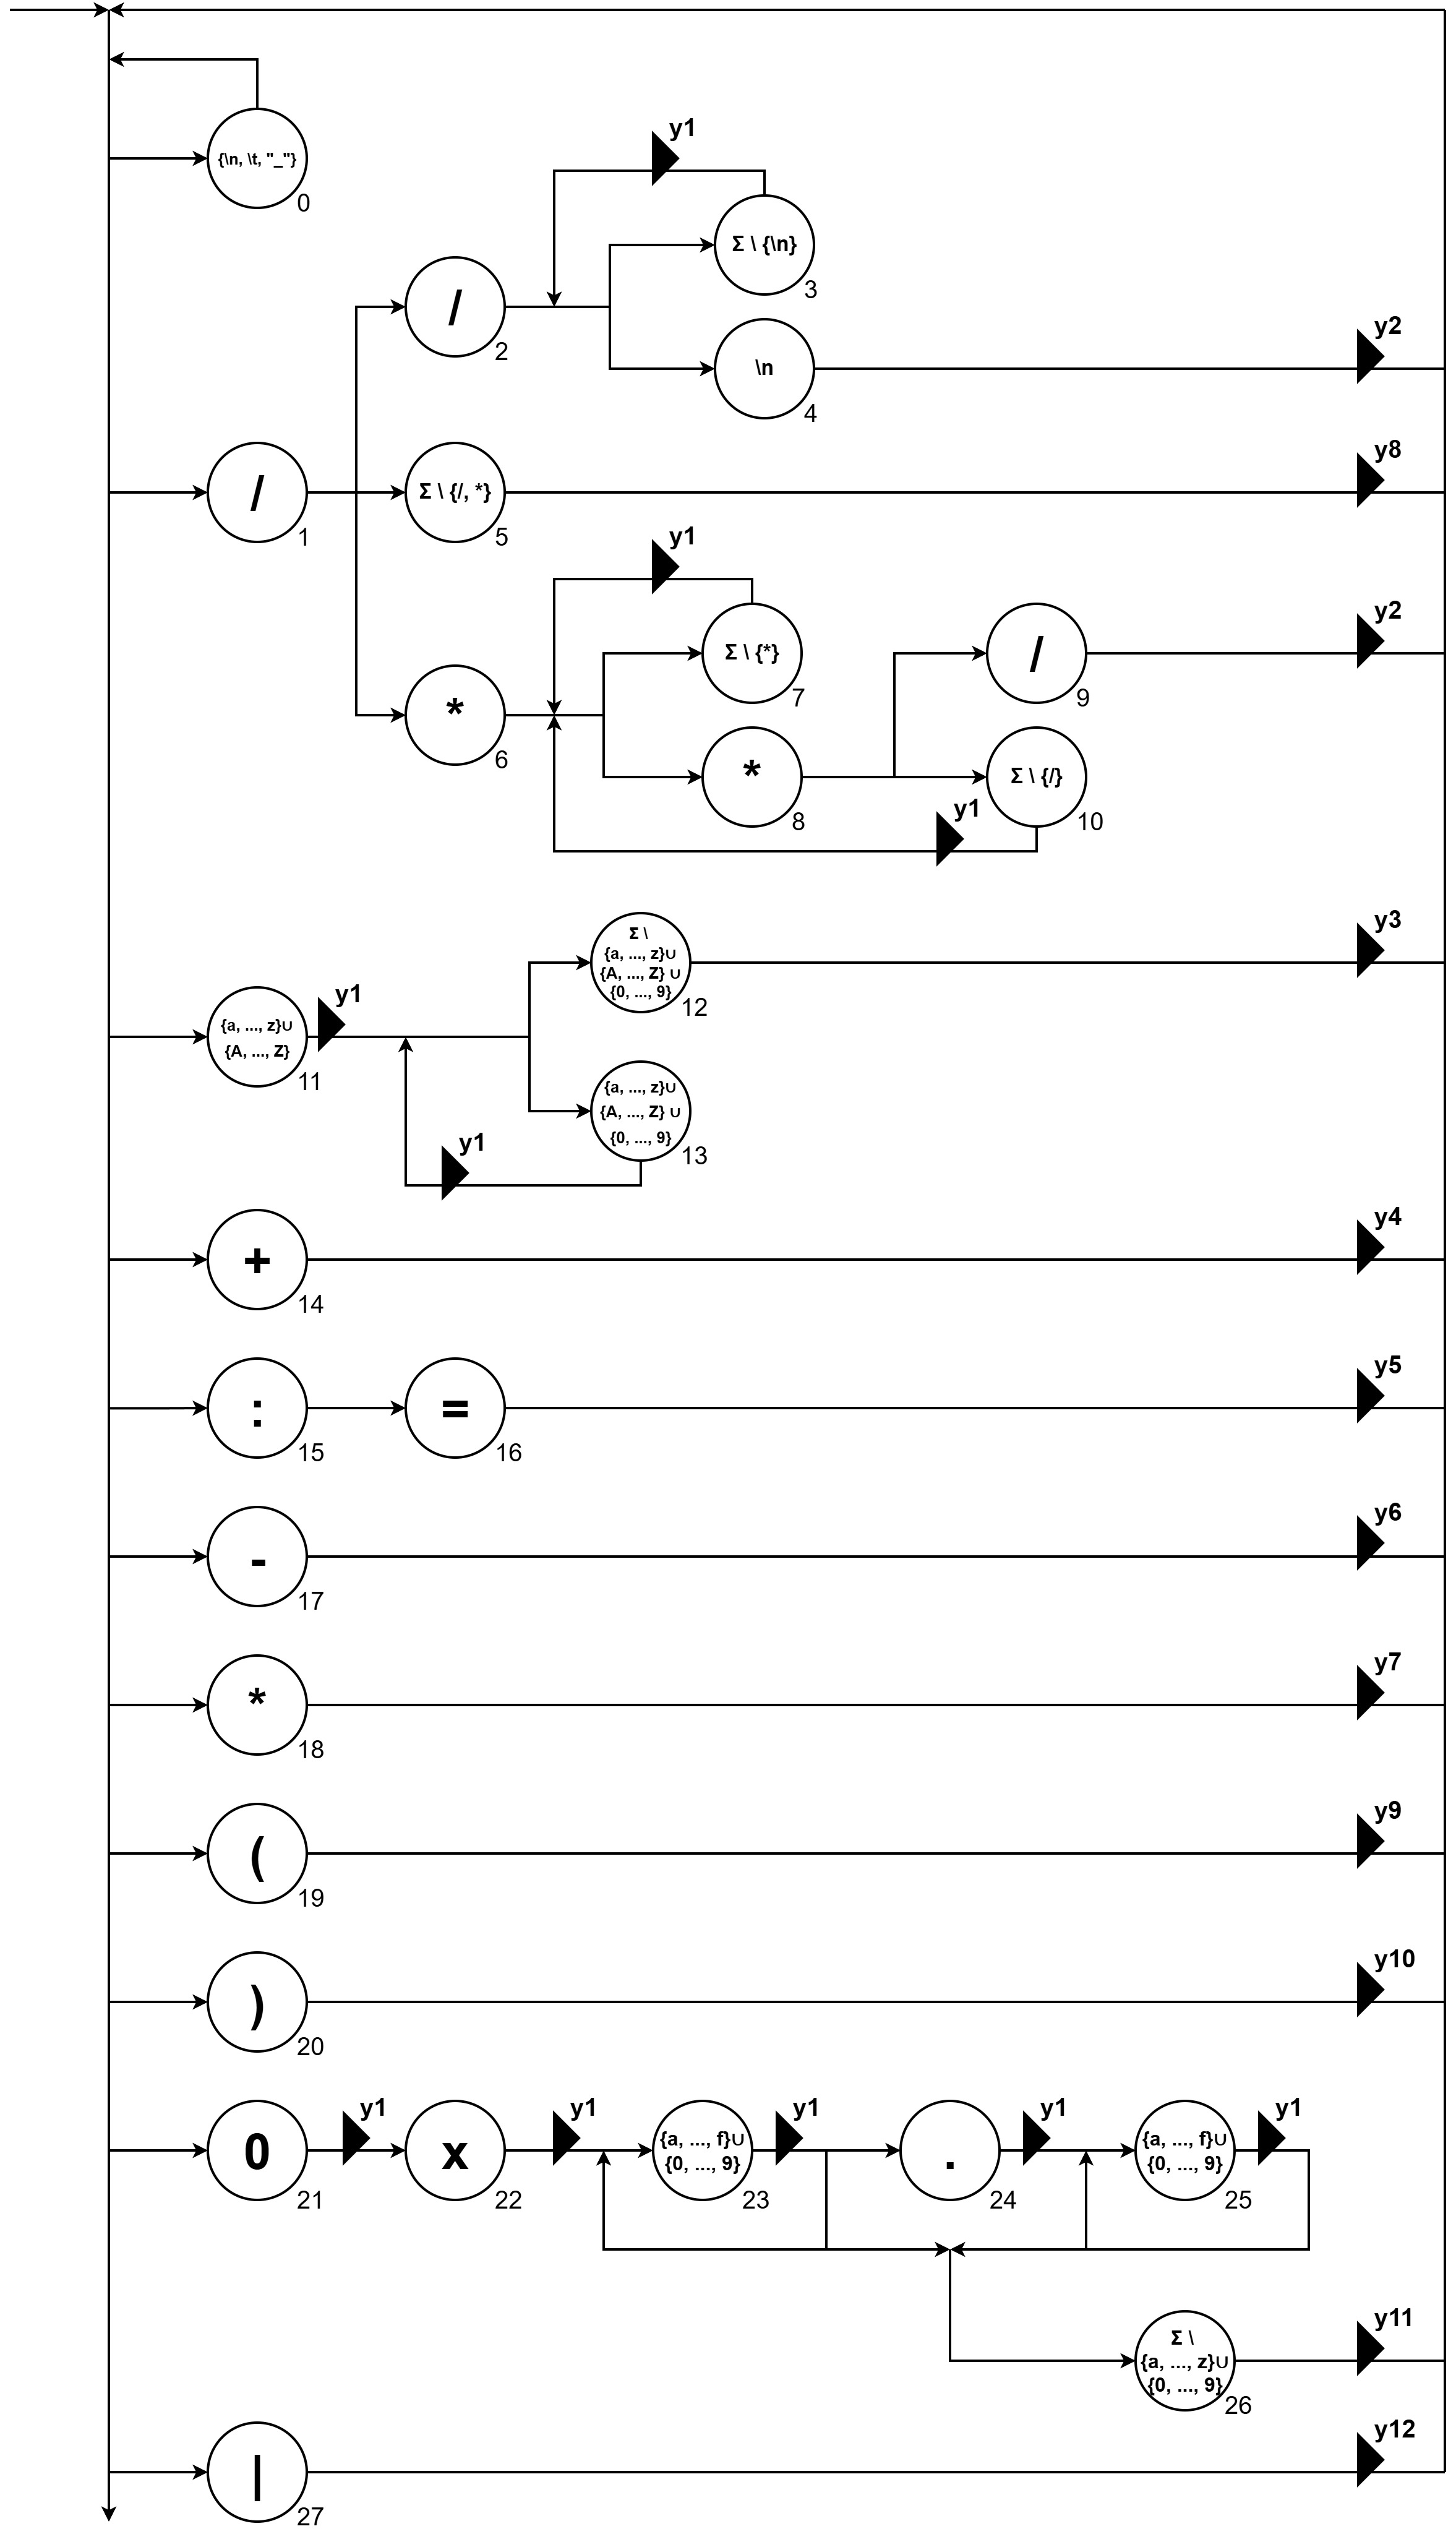
\includegraphics[width=0.7\linewidth]{Синтаксическая диаграмма.jpg}
    \caption{\centering Синтаксическая диаграмма лексического анализатора}
\end{figure}

Действия используемые в синтаксической диаграмме:
\begin{itemize}
    \item y1 -- записать символ в буфер
    \item y2 -- очистить буфер
    \item y3 -- выдать лексему <id, значение> и очистить буфер
    \item y4 -- выдать лексему <arithmetic, ''+''>
    \item y5 -- выдать лексему <assign, '':=''>
    \item y6 -- выдать лексему <arithmetic, ''-''>
    \item y7 -- выдать лексему <arithmetic, ''*''>
    \item y8 -- выдать лексему <arithmetic, ''/''>
    \item y9 -- выдать лексему <left\_bracket, ''(''>
    \item y10 -- выдать лексему <right\_bracket, '')''>
    \item y11 -- выдать лексему <const, значение> и очистить буфер
    \item y12 -- выдать лексему <separator, ''|''>
\end{itemize}

\newpage
\section{Особенности реализации}
\subsection{Структуры данных}
\subsubsection{Класс лексем}
С помощью класса Lexem в программе реализовано задание типов лексем и хранение выделяемых лексическим анализатором лексем. Также данный класс реализует отслеживание уже добавленных идентификаторов -- если добавляемый идентификатор уже был добавлен ранее, то ему присвоится такой же номер, как и предыдущему. Код объявления данного класса представлен на листинге 1.
\footnotesize{
\begin{lstlisting}[language=C++, caption = {Код класса Lexem}]
class Lexem {
private:
	static map<string, int> type_to_int;
	static map<int, string> int_to_type;
	static map<string, string> type_to_rus;
	static map<string, int> ids;
	static int count_ids;
	int type;
	string token;
	
public:
	static void set_types(initializer_list<pair<string, string>>);
	static void clr_ids();
	Lexem(string, string);
	string get_token();
	string get_type(bool = false);
	string get_value();
};
\end{lstlisting}
}
\small

Для задания доступных типов лексем используется статический метод set\_types. Для каждого типа задаётся два названия: английское (для внутреннего использования) и русское (для вывода в таблицу лексем). Также для каждого добавляемого типа создаётся его числовое представление, а сами названия типов хранятся в словаре, далее в самом классе используются только числовые представления. Данная манипуляция позволяет не хранить для каждой лексемы строку с её типом, что существенно уменьшает количество потребляемой памяти при анализе текстов с большим количеством лексем.

Вход: последовательность пар <string, string> -- <Английское название, Русское название>.

Выход: класс Lexem с заданными возможными типами лексем.

Код данного метода представлен на листинге 2.
\footnotesize{
\begin{lstlisting}[language=C++, caption = {Код метода set\_types}]
void Lexem::set_types(initializer_list<pair<string, string>> new_types) {
	int count_types = 0;
	for (pair<string, string> t : new_types) {
		auto result = Lexem::type_to_int.try_emplace(t.first, count_types);
		if (result.second) {
			Lexem::int_to_type.emplace(count_types, t.first);
			Lexem::type_to_rus.emplace(t.first, t.second);
			count_types++;
		}
	}
}
\end{lstlisting}
}
\small

Для создания новой лексемы используется конструктор класса Lexem. Если лексема является идентификатором, то проверяется существует ли уже идентификатор с таким названием, если не существует, то в словарь содержащий номера для всех уникальных идентификаторов добавляется новое значение. Код данного конструктора расположен на листинге 3.

Вход: строка, содержащая тип лексемы, и строка, представляющая токен лексемы из заданного текста.

Выход: новая лексема с заданным токеном, типом, а также значением, если тип -- идентификатор.

\footnotesize{
\begin{lstlisting}[language=C++, caption = {Код конструктора класса Effect}]
Lexem::Lexem(string type_str, string token) {
	this->token = token;
	this->type = Lexem::type_to_int[type_str];

	if (this->type == 0) {
		auto result = Lexem::ids.try_emplace(this->token, Lexem::count_ids);
		if (result.second) {
			Lexem::count_ids += 1;
		}
	}
}
\end{lstlisting}
}
\small


\subsubsection{Класс эффектов}
Данный класс является обёрткой для функций реализующих выполнение различных действий при переходе между узлами синтаксической диаграммы. Наличие данного класса позволяет использовать вызов объекта как функции для выполнения различных действий. Использование данного класса на данный момент не имеет большой выгоды, но при дальнейшем развитии программы может существенно помочь для реализации более сложных эффектов. Код объявления данного класса представлен на листинге 4.

\footnotesize{
\begin{lstlisting}[language=C++, caption = {Код класса Effect}]
class Effect {
private:
	function<void()> func;
public:
	Effect(function<void()>);
	void apply();
};
\end{lstlisting}
}
\small

Конструктор класса Effect позволяет создать обёртку вокруг лямбда-функции и в дальнейшем вызывать полученный экземпляр как данную функцию.

Вход: функция, не имеющая аргументов и не возвращающая значения.

Выход: полученная функция обёрнутая в объект класса Effect.

Также для данного класса был переопределён оператор вызова без аргументов, что позволяет запускать выполнение функции эффекта, через вызов самого эффекта.

Вход: функция данного эффекта.

Выход: выполнение функции эффекта.

Коды определения конструктора класса Effect и переопределения оператора можно увидеть на листинге 5.

\footnotesize{
\begin{lstlisting}[language=C++, caption = {Код конструктора класса Effect}]
Effect::Effect(function<void()> func) {
	this->func = func;
}

void Effect::operator()() {
	this->func();
}
\end{lstlisting}
}
\small

\subsubsection{Класс узла диаграммы}
Основой реализации лексического анализатора в разработанной программе является использование конечного автомата, соответствующего созданной синтаксической диаграмме. Для представления в программе диаграммы и её узлов используется один класс Node, конструктор которого даёт возможность добавлять новые узлы в диаграмму, а статические методы и поля класса позволяют использовать сам класс как представление всей синтаксической диаграммы. Далее на листинге 6 представлен код объявления данного класса.

\footnotesize{
\begin{lstlisting}[language=C++, caption = {Код класса Node}]
class Node {
private:
	function<bool(char)> match;
	vector<Node*> next_nodes;
	vector<Effect*> current_effects;
	string name;

public:
	static Node* start_node;
	static Node* error_node;
	static Effect* error_effect;
	static Node* current_node;

	static deque<char> data;
	static char prev_char;
	static string buffer;
	static vector<pair<string, string>> errors;
	static vector<Lexem*> table;
	
	void set_params(function<bool(char)>, vector<Node*>, vector<Effect*>, string);
	void apply_effects();
	static bool go_to_next(bool);
	static pair<vector<Lexem*>, vector<pair<string, string>>> analyze(string, bool = false , bool = false);
};
\end{lstlisting}
}
\small

\paragraph{Назначение полей класса}
\begin{enumerate}[label=]
    \item Обычные поля (для узла диаграммы):
    \begin{itemize}
        \item \textbf{match} -- функция, возвращающая true, если переход в данный узел по текущему символу возможен;
        \item \textbf{next\_nodes} -- вектор указателей на следующие узлы диаграммы;
        \item \textbf{current\_effects} -- вектор эффектов, применяемых при переходе в данный узел;
        \item \textbf{name} -- название узла (используется при отладке).
    \end{itemize}
    \item Статические поля (для диаграммы):
    \begin{itemize}
        \item \textbf{start\_node} -- начальный узел диаграммы;
        \item \textbf{error\_node} -- узел обработчика ошибки, предназначенный для сбора символов токена ошибки;
        \item \textbf{error\_effect} -- эффект, применяемый при попадании в узел обработчика ошибки;
        \item \textbf{current\_node} -- текущий узел;
        \item \textbf{data} -- двухсторонняя очередь из символов, был выбран такой контейнер для быстрого взятия первого символа текста и более эффективного хранения данных по сравнению с контейнером list;
        \item \textbf{prev\_char} -- предыдущий взятый символ, используется для правильной обработки ошибки незакрытого многострочного комментария;
        \item \textbf{buffer} -- строка представляющая буфер, в котором находятся записанные по мерепрохождения узлов значения;
        \item \textbf{errors} -- вектор пар строк <Ошибочный токен, Описание ошибки>;
        \item \textbf{table} -- вектор указателей на найденные лексемы, хранение указателей позволяет не создавать заново сложные объекты базовых лексем (операторы, скобки, разделитель).
    \end{itemize}
\end{enumerate}

\paragraph{Обычные методы класса (для узла)\\[1em]}
В общем случае нельзя задать следующие узлы при создании нового узла, так как, например, при создании петель следующим узлом будет являться данный узел, указатель на который неопределён. Поэтому в определении класса отсутствует конструктор и используется конструктор по умолчанию, который инициализирует нестатические поля из базовыми значениями, а уже определение параметров узла происходит с помощью вызова метода set\_params.

Метод set\_params реализует инициализацию параметров узла вместо конструктора. Код данного метода расположен на листинге 7.

Вход: функция, определяющая допустимость перехода в данный узел; следующие узлы; эффекты данного узла; имя узла.

Выход: объект узла синтаксической диаграммы  с полностью определёнными полями.
\footnotesize{
\begin{lstlisting}[language=C++, caption = {Код метода set\_params}]
void Node::set_params(function<bool(char)> match, vector<Node*> next_nodes, vector<Effect*> current_effects, string name) {
	this->match = match;
	this->next_nodes = next_nodes;
	this->current_effects = current_effects;
	this->name = name;
}
\end{lstlisting}
}
\small

После выбора следующего узла, в который должна перейти работа при взятии следующего символа входного текста, происходит выполнение действий (эффектов), определённых для следующего узла. Данный функционал реализован в методе apply\_effects, который вызывает каждый эффект данного узла.

Вход: узел с определёнными для него эффектами при переходе.

Выход: выполнение эффектов

Код метода apply\_effects представлен на листинге 8.
\footnotesize{
\begin{lstlisting}[language=C++, caption = {Код метода apply\_effects}]
void Node::apply_effects() {
	for (Effect* eff : this->current_effects) {
		(*eff)();
	}
}
\end{lstlisting}
}
\small

\paragraph{Статические методы класса (для всей диаграммы)\\[1em]}
После формирования всех узлов, составляющих синтаксическую диаграмму, и задания связей между ними можно начинать работу с самой диаграммой. Для реализации перехода в следующий узел был создан статический метод go\_to\_next. Данный метод при условии наличия символов в цепочке берёт следующий символ, выбирает узел в который будет совершён переход исходя из взятого символа и применяет эффекты, соответствующие новому узлу. В случае если не был найден подходящий узел, происходит переход в узел обработчика ошибок и применяются его эффекты.

Вход: параметры текущего узла и входная цепочка 

Выход: Изменённое состояние синтаксической диаграммы (новый текущий узел), выполненные эффекты следующего узла и булевое значение, означающее наличие символов в цепочке.

Код метода go\_to\_next представлен на листинге 9.
\footnotesize{
\begin{lstlisting}[language=C++, caption = {Код метода go\_to\_next}]
bool Node::go_to_next() {
	if (!Node::data.empty()) {
		char c = Node::data.front();
		for (Node* next_node : current_node->next_nodes) {
			if (next_node->match(c)) {
				current_node = next_node;
				current_node->apply_effects();
				return true;
			}
		}
		current_node = error_node;
		current_node->apply_effects();
		return true;
	}
	return false;
}
\end{lstlisting}
}
\small

Лексический анализ осуществляется с помощью последовательного взятия следующего символа входной цепочки, перехода в узел, соответствующий взятому символу, и выполнения действий при переходе узел пока не закончатся все символы во входной цепочке. Данный алгоритм реализован в методе analyze. 

Этот метод производит очистку контекста (таблицы лексем и ошибок) предыдущих лексических анализов при необходимости, последовательно переходит к следующему узлу и выполняет эффекты пока во входной цепочке есть символы, а также выявляет ошибку незаконченного многострочного комментария.

Вход: объект синтаксической диаграммы, входная цепочка символов и флаг очистки контекста.

Выход: таблица лексем и таблица ошибок, полученные в результате лексического анализа.

Код данного метода представлен на листинге 10.

\footnotesize{
\begin{lstlisting}[language=C++, caption = {Код метода analyze}]
pair<vector<Lexem*>, vector<pair<string, string>>> Node::analyze(string str, bool with_context) {

	Node::data = deque<char>(str.begin(), str.end());
	Node::current_node = Node::start_node;

	if (!with_context) {
		table.clear();
		errors.clear();
	}
	while (Node::go_to_next(debug)) { };
	if (!Node::buffer.empty()) {
		Node::buffer.pop_back();
		Node::errors.push_back({ Node::buffer, "Многострочный комменатрий не завершён"});
		Node::buffer.clear();
	}
	return { table, errors };
}
\end{lstlisting}
}
\small

\subsection{Определение параметров лексического анализатора}
Вся настройка лексического анализатора происходит с помощью работы с методами и полями ранее представленных классов в функции main, только после настройки запуск лексического анализатора считается допустимым.

Далее представлена настройки отдельных компонентов лексического анализатора.
\paragraph{Настройка лексем\\[1em]}
Первым делом при настройке лексического анализатора нужно определить входной язык и лексемы, которые он сможет выявлять. Далее на листинге 11 представлено определение символов входного языка, задание допустимых типов лексем и создание базовых лексем, чьи токены постоянны.
\footnotesize{
\begin{lstlisting}[language=C++, caption = {Определение входного языка и лексем}]
string alph = "abcdefghijklmnopqrstuvwxyzABCDEFGHIJKLMNOPQRSTUVWXYZ1234567890+-*/:=|().\n\t ";

// Задание типов лексем
Lexem::set_types({ 
	{"id", "Идентификатор"}, 
	{"arithmetic", "Арифметический оператор"}, 
	{"assign", "Знак присваивания"}, 
	{"left_bracket", "Левая скобка"}, 
	{"right_bracket", "Правая скобка"}, 
	{"const", "Константа"}, 
	{"separator", "Разделитель"}
	});

// Создание базовых лексем
Lexem* lexem_plus = new Lexem("arithmetic", "+");
Lexem* lexem_minus = new Lexem("arithmetic", "-");
Lexem* lexem_mult = new Lexem("arithmetic", "*");
Lexem* lexem_div = new Lexem("arithmetic", "/");
Lexem* lexem_assign = new Lexem("assign", ":=");
Lexem* lexem_lt_bracket = new Lexem("left_bracket", "(");
Lexem* lexem_rt_bracket = new Lexem("right_bracket", ")");
Lexem* lexem_sep = new Lexem("separator", "|");
\end{lstlisting}
}
\small

\paragraph{Создание эффектов\\[1em]}
После определения лексем определяются все возможные эффекты при переходе в узлы синтаксической диаграммы. Каждый эффект создаётся с помощью конструктора класса Effect с аргументов соответствующим функции выполняющей действия эффекта. Код создания эффектов представлен на листинге 12.

\footnotesize{
\begin{lstlisting}[language=C++, caption = {Код класса Effect}]
// удаление первого символа
Effect shift([]() { 
	Node::prev_char = Node::data.front(); 
	Node::data.pop_front();
	});
// очистка буфера
Effect clr_buf([]() { Node::buffer.clear(); });
// удаление последнего символа буфера
Effect pop_back_buf([]() { Node::buffer.pop_back(); });
// добавление ошибки
Effect add_error([&cur_group]() {
	string err_com = get_err_comment(cur_group);
	
	Node::errors.push_back({ Node::buffer, err_com });
	});
// инкрементирование счётчика символов идентфиикатора
Effect add_char_in_id([&cur_group, &count_chars_identifier]() {  
	if (++count_chars_identifier > 15) {
		cur_group = Group::id_over;
	}
	});
// инкрементирование счётчика символов константы
Effect add_char_in_number([&cur_group, &count_chars_number]() {
	if (++count_chars_number > 15) {
		cur_group = Group::number_over;
	}
	});

// Основные эффекты
Effect y1([]() { Node::buffer.push_back(Node::data.front());});
Effect y3([]() { Node::table.push_back(new Lexem("id", Node::buffer)); });
Effect y4([&lexem_plus]() { Node::table.push_back(lexem_plus); });
Effect y5([&lexem_assign]() { Node::table.push_back(lexem_assign); });
Effect y6([&lexem_minus]() { Node::table.push_back(lexem_minus); });
Effect y7([&lexem_mult]() { Node::table.push_back(lexem_mult); });
Effect y8([&lexem_div]() { Node::table.push_back(lexem_div); });
Effect y9([&lexem_lt_bracket]() { Node::table.push_back(lexem_lt_bracket); });
Effect y10([&lexem_rt_bracket]() { Node::table.push_back(lexem_rt_bracket); });
Effect y11([]() { Node::table.push_back(new Lexem("const", Node::buffer)); });
Effect y12([&lexem_sep]() { Node::table.push_back(lexem_sep); });

// Эффекты для отслеживания группы узлов
Effect in_ws([&cur_group, &count_chars_identifier, &count_chars_number]() {
	cur_group = Group::all; 
	count_chars_identifier = 0; 
	count_chars_number = 0;
	});
Effect in_comment([&cur_group]() { cur_group = Group::comment; });
Effect in_mr_comment([&cur_group]() { cur_group = Group::mr_comment; });
Effect in_id([&cur_group]() { cur_group = Group::id; });
Effect in_assign([&cur_group]() { cur_group = Group::assign; });
Effect in_number([&cur_group]() { cur_group = Group::number; });
\end{lstlisting}
}
\small

\paragraph{Настройка типов ошибок\\[1em]}
Для вывода комментариев к находимым во время лексического анализа ошибкам узлы синтаксической диаграммы были разбиты на следующие группы:
\begin{itemize}
    \item общая группа;
    \item обработка однострочного комментария;
    \item обработка многострочного комментария;
    \item обработка идентификатора;
    \item обработка идентификатора превышающего 15 символов;
    \item обработка оператора присваивания;
    \item обработка числа;
    \item обработка числа превышающего 15 символов;
\end{itemize}

Стоит заметить, что разбиение узлов на данные группы не является статичным, а зависит от самого узла и от текущего количества символов в обрабатываемом идентификаторе или числе. Переход в другую группу при переходе между узлами производится с помощью выполнения соответствующего эффекта для определённой группы.

Для каждой группы были определены комментарии к ошибкам, возникающим в данных группах. Далее в листинге 13 представлен код объявления групп и определение комментариев к ошибкам.
\footnotesize{
\begin{lstlisting}[language=C++, caption = {Создание групп и определение комментариев}]
enum class Group {
	all,
	comment,
	mr_comment,
	id,
	id_over,
	assign,
	number,
	number_over
};

string get_err_comment(Group cur_group) {
	switch (cur_group)
	{
	case Group::comment: return "Неизвестные символы в комментарии";
	case Group::mr_comment: return "Неизвестные символы в многострочном комментарии";
	case Group::id: return "Неправильное название идентификатора";
	case Group::id_over: return "Идентификатор содержит больше 15 символов";
	case Group::number: return "Неверный формат вещественной константы";
	case Group::number_over: return "Вещественная константа содержит больше 15 символов";
	default:
        return "Неизвестная лексема";
	}
}
\end{lstlisting}
}
\small

\paragraph{Создание узлов диаграммы\\[1em]}
На листинге 14 можно увидеть создание узлов разработанной синтаксической диаграммы лексического анализатора. Для каждого узла задаётся предикат возможности перехода в данный узел, следующие узлы, эффекты применяемые при переходе в данный узел, и его порядковый номер в качестве имени. 

Отдельно было создано два узла для обработки ошибок: узел обработчика ошибки последовательно собирает символы составляющие токен ошибки, а узел сборщика ошибки по текущей группе узлов определяет тип ошибки и возвращает управление в соответствующий следующему символу узел. Также следует обратить внимание, что предикат возможности перехода в узел сборщика ошибки не статичный, а зависит от текущей группы, например, для группы узлов обрабатывающих однострочный комментарий предикатом будет результат проверки принадлежности символа к буквам, цифрам или точке, а для обрабатывающих многострочные комментарии -- результат проверки того, что текущий символ равен ''/'', а предыдущий -- ''*''.
\footnotesize{
\begin{lstlisting}[language=C++, caption = {Код создания узлов диаграммы}]
// Создание узлов диаграммы
vector<Node> nodes(28);
vector<Node*> nodes_first({ &nodes[0], &nodes[1], &nodes[11], &nodes[14], &nodes[15], &nodes[17], &nodes[18], &nodes[19], &nodes[20], &nodes[21], &nodes[27] });
nodes[0].set_params([](char c) {return is_ws_char(c); }, nodes_first, { &clr_buf, &in_ws, &shift }, "0");
nodes[1].set_params(is_slash, { &nodes[2], &nodes[5], &nodes[6] }, { &clr_buf, &shift }, "1");
nodes[2].set_params(is_slash, { &nodes[3], &nodes[4] }, { &in_comment, &shift }, "2");
nodes[3].set_params([](char c) {return c != '\n'; }, { &nodes[3], &nodes[4] }, { &y1, &shift }, "3");
nodes[4].set_params([](char c) {return c == '\n'; }, nodes_first, { &shift }, "4");
nodes[5].set_params([](char c) {return c != '/' && c != '*' && in_alph(c); }, nodes_first, { &y8 }, "5");
nodes[6].set_params([](char c) {return c == '*'; }, { &nodes[7], &nodes[8] }, { &in_mr_comment, &shift }, "6");
nodes[7].set_params([](char c) {return c != '*'; }, { &nodes[7], &nodes[8] }, { &y1, &shift }, "7");
nodes[8].set_params([](char c) {return c == '*'; }, { &nodes[9], &nodes[10] }, { &y1, &shift }, "8");
nodes[9].set_params(is_slash, nodes_first, { &pop_back_buf, &shift}, "9");
nodes[10].set_params([](char c) {return c != '/'; }, { &nodes[7], &nodes[8] }, { &in_mr_comment, &y1 }, "10");
nodes[11].set_params([](char c) {return 'a' <= c && c <= 'z' || 'A' <= c && c <= 'Z'; }, { &nodes[12], &nodes[13] }, { &clr_buf, &in_id, &y1, &shift, &add_char_in_id }, "11");
nodes[12].set_params([](char c) {return not ('a' <= c && c <= 'z' || 'A' <= c && c <= 'Z' || '0' <= c && c <= '9') && in_alph(c); }, nodes_first, {&y3 }, "12");
nodes[13].set_params([&count_chars_identifier](char c) {return ('a' <= c && c <= 'z' || 'A' <= c && c <= 'Z' || '0' <= c && c <= '9') && count_chars_identifier <= 15; }, { &nodes[12], &nodes[13] }, { &y1, &shift, &add_char_in_id }, "13");
nodes[14].set_params([](char c) {return c == '+'; }, nodes_first, { &clr_buf, &in_ws, &y4, &shift }, "14");
nodes[15].set_params([](char c) {return c == ':'; }, { &nodes[16] }, { &clr_buf, &in_assign, &shift }, "15");
nodes[16].set_params([](char c) {return c == '='; }, nodes_first, { &y5, &in_ws, &shift }, "16");
nodes[17].set_params([](char c) {return c == '-'; }, nodes_first, { &clr_buf, &in_ws, &y6, &shift }, "17");
nodes[18].set_params([](char c) {return c == '*'; }, nodes_first, { &clr_buf, &in_ws, &y7, &shift }, "18");
nodes[19].set_params([](char c) {return c == '('; }, nodes_first, { &clr_buf, &in_ws, &y9, &shift }, "19");
nodes[20].set_params([](char c) {return c == ')'; }, nodes_first, { &clr_buf, &in_ws, &y10, &shift }, "20");
nodes[21].set_params([](char c) {return c == '0'; }, { &nodes[22] }, { &clr_buf, &in_number, &y1, &shift, &add_char_in_number }, "21");
nodes[22].set_params([](char c) {return c == 'x'; }, { &nodes[23] }, { &y1, &shift, &add_char_in_number }, "22");
nodes[23].set_params([&count_chars_number](char c) {return ('a' <= c && c <= 'f' || '0' <= c && c <= '9') && count_chars_number <= 15; }, { &nodes[23], &nodes[24], &nodes[26] }, { &y1, &shift, &add_char_in_number }, "23");
nodes[24].set_params([&count_chars_number](char c) {return c == '.' && count_chars_number <= 15; }, { &nodes[25] }, { &y1, &shift, &add_char_in_number }, "24");
nodes[25].set_params([&count_chars_number](char c) {return ('a' <= c && c <= 'f' || '0' <= c && c <= '9') && count_chars_number <= 15; }, { &nodes[25], &nodes[26] }, { &y1, &shift, &add_char_in_number }, "25");
nodes[26].set_params([](char c) {return not in_num_chars(c); }, nodes_first, {&y11, &clr_buf, &in_ws }, "26");
nodes[27].set_params([](char c) {return c == '|'; }, nodes_first, { &clr_buf, &in_ws, &y12, &shift }, "27");

// Узел сборщика ошибки
Node error_builder_node;
error_builder_node.set_params(
	[&cur_group](char c) { 
		switch (cur_group)
		{
		case Group::id: return not is_id_char(c) && in_alph(c);
		case Group::id_over: return not is_id_char(c) && in_alph(c);
		case Group::comment: return c == '\n';
		case Group::mr_comment: 
			if (c == '/' && Node::prev_char == '*') {
				Node::buffer.pop_back();
				return true;
			}
			return false;
			
		case Group::number: return !in_num_chars(c);
		case Group::number_over: return !in_num_chars(c);
		default: return in_alph(c);
		}
	}, nodes_first, { &add_error, &clr_buf, &in_ws }, "error_builder");

// Узел обработчика ошибки
Node::error_node = new Node();
vector<Node*> nodes_from_error = nodes_first;
nodes_from_error.push_back(Node::error_node);
Node::error_node->set_params([](char c) {return false; }, { &error_builder_node}, { &y1, &shift }, "error");
\end{lstlisting}
}
\small

\subsection{Функция обработки пользовательского ввода}
После настройки анализатора его можно запускать с заданием обрабатываемого текста. Функционал обработки пользовательского ввода реализован в функции input\_loop, которая предлагает пользователю варианты действий и выполняет действие исходя из ввода пользователя.

Данная функция предоставляет пользователю следующие меню:
\begin{enumerate}
    \item \textbf{Меню чтения текста}. Пользователю предоставляется выбор того как ввести код программы для последующей обработки: ручной ввод или ввод из файла. После получения кода программы пользователю предлагается вывести её код и после этого происходит переход в главное меню.
    \item \textbf{Главное меню}. В данном меню пользователю даётся возможность выполнить следующие действия:
    \begin{itemize}
        \item провести лексический анализ текста;
        \item очистить контекст;
        \item вывести код программы;
        \item ввести новый код программы;
        \item выход
    \end{itemize}
    После выбора пользователя программы выполняет соответствуеющее действие и возвращает пользователя обратно в главное меню. Под очисткой контекста подразумевается удаление содержимого таблиц лексем и ошибок. Наличие возможности выполнения анализа другого кода без очистки контекста может быть полезно для анализа нескольких исходных кодов как модулей одной программы.
\end{enumerate}

Код определения данной функции представлен на листинге 15. 
\footnotesize{
\begin{lstlisting}[language=C++, caption = {Код функции пользовательского ввода}]
void input_loop() {
    cout << "===== Лексический анализатор кода =====" << endl;
    string user_input;
    string data;
    while (true) {
        cout << "\nВыберите действие:\n\t[1] Ввести код программы\n\t[2] Прочитать код программы из файла\n\t[exit] Выход" << endl;
        getline(cin, user_input);
        if (user_input == "1") {
            cout << "\nВведите код программы:" << endl;
            getline(cin, data);
        }
        else if (user_input == "2") {
            bool in_reading = true;
            bool exit = false;
            while (in_reading) {
                string path;
                cout << "\nВведите путь к файлу ('exit' чтобы отменить):\n";
                getline(cin, path);
                if (path == "exit") { exit = true; in_reading = false; }
                else {
                    ifstream file(path);
                    if (file.is_open()) {
                        data = string(istreambuf_iterator<char>(file), istreambuf_iterator<char>());
                        in_reading = false;
                        cout << "\033[92mФайл прочитан.\033[0m\n\tКоличество строк - " << count(data.begin(), data.end(), '\n') + 1 << "\n\tКоличество символов - " << utf8_length(data) << endl;
                        bool in_print_file = true;
                        while (in_print_file) {
                            cout << "\nВывести содержимое файла? [Да / Нет]" << endl;
                            getline(cin, user_input);
                            if (user_input == "Да" || user_input == "да" || user_input == "Д" || user_input == "д") {
                                cout << "\n\033[94m(Начало программы)\033[0m\n" << data << "\n\033[94m(Конец программы)\033[0m" << endl;
                                in_print_file = false;
                            }
                            else if (user_input == "Нет" || user_input == "нет" || user_input == "Н" || user_input == "н") {
                                in_print_file = false;
                            }
                            else {
                                cout << "\033[91mВыбор не распознан. Повторите попытку.\033[0m" << endl;
                                continue;
                            }
                        }
                    }
                    else {
                        cout << "\033[91mВведённый путь не найден. Повторите попытку.\033[0m" << endl;
                    }
                }
            }
            if (exit) { continue; };
        }
        else if (user_input == "exit"){
            break;
        }
        else{
            cout << "\033[91mВыбор не распознан. Повторите попытку.\033[0m" << endl;
            continue;
        }
        bool in_output = true;
        bool exit = false;
        while (in_output) {
            cout << "\nВыберите действие:\n\t[1] Провести лексический анализ кода программы\n\t[2] Очистить контекст\n\t[3] Вывести код программы\n\t[4] Ввести новый код программы\n\t[exit] Выход" << endl;
            getline(cin, user_input);
            if (user_input == "1") {
                print_analysis_result(Node::analyze(data + "\n", false, true));
            }
            else if (user_input == "2") {
                Node::errors.clear();
                Node::table.clear();
                Lexem::clr_ids();
            }
            else if (user_input == "3") {
                cout << "\n\033[94m(Начало программы)\033[0m\n" << data << "\n\033[94m(Конец программы)\033[0m" << endl;
            }
            else if (user_input == "4") {
                in_output = false;
            }
            else if (user_input == "exit") {
                exit = true;
                in_output = false;
            }
            else {
                cout << "\033[91mВыбор не распознан. Повторите попытку.\033[0m" << endl;
                continue;
            }
        }
        if (exit) { break; };
    }
    cout << "Выход из программы." << endl;
}
\end{lstlisting}
}
\small
\newpage
\section{Результаты работы программы}
Далее представлены таблица лексем и ошибки при проведение лексического анализа различных текстов.

На рисунке 3 представлен вывод для следующего текста:
\begin{verbatim}
    /*Многострочный
    комменатрий*/
    var1:=0x0.e12fa0|
	       var2 := var1 * (0x15 + 0xf3.91)| \\ обычный комментарий
\end{verbatim}
\begin{figure}[H]
    \centering
    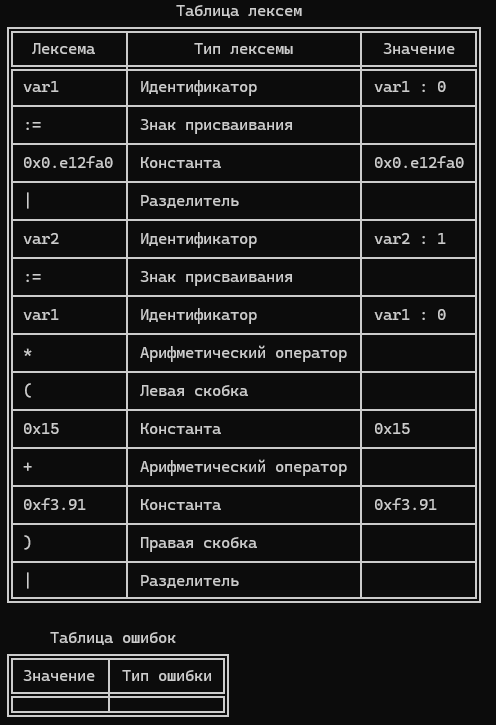
\includegraphics[width=0.5\linewidth]{Пример 1.png}
    \caption{\centeringРезультат лексического анализа примера 1}
\end{figure}

На рисунке 4 представлен вывод для следующего текста, содержащего неправильно записанные числа и незакрытый многострочный комментарий:
\begin{verbatim}
    var1:=0x0.E12fA0 + 0x0.1.fa4
    /*Незакрытый
    многострочный *
    комментарий
\end{verbatim}
\begin{figure}[H]
    \centering
    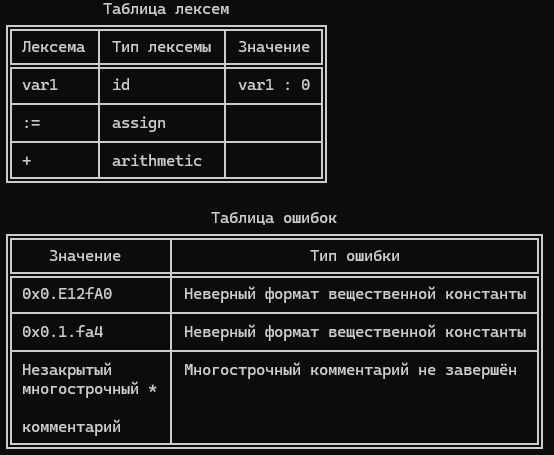
\includegraphics[width=0.5\linewidth]{Пример 2.png}
    \caption{\centeringРезультат лексического анализа примера 2}
\end{figure}

На рисунке 5 представлен вывод для следующего текста, содержащего идентификатор и константу, чьи длины больше 15 символов:
\begin{verbatim}
    longlongvariable := 0x0.ff1
    var := 0x123456789.abcdef
\end{verbatim}
\begin{figure}[H]
    \centering
    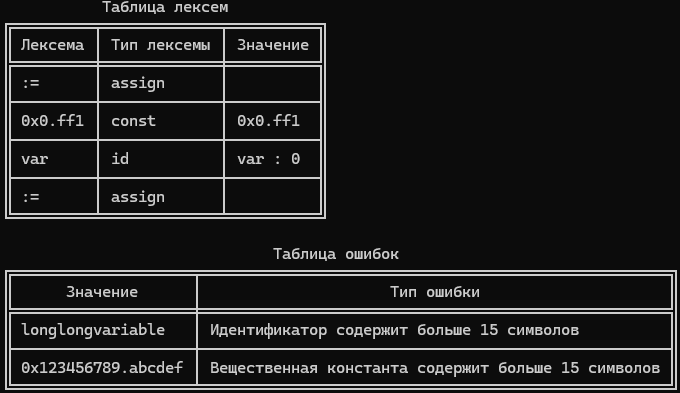
\includegraphics[width=0.6\linewidth]{Пример 4.png}
    \caption{\centeringРезультат лексического анализа для примера 4}
\end{figure}

На рисунке 6 представлен вывод для следующего текста, содержащего сочетание символов ''::=='' и идентификатор начинающийся с цифры:
\begin{verbatim}
    varNormal ::== 0x57.6f
    1varError := varNormal * 0x0.1
\end{verbatim}
\begin{figure}[H]
    \centering
    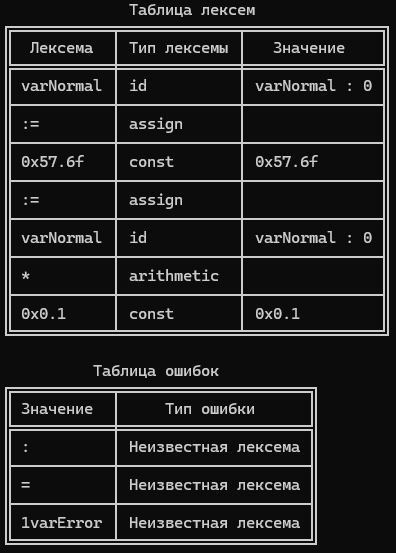
\includegraphics[width=0.5\linewidth]{Пример 5.png}
    \caption{\centeringРезультат лексического анализа для примера 5}
\end{figure}

\newpage
\section*{Заключение}
В ходе выполнения данной лабораторной работы был разработан лексический анализатор, позволяющий выделять лексемы и обнаруживать ошибки в тексте написанном на заданном языке, который содержит:
\begin{itemize}
    \item символы латиницы;
    \item идентификаторы, состоящие из не более чем 15 символов;
    \item вещественные шестнадцатеричные константы, состоящие из не более чем 15 символов;
    \item операторы '+', '-', '*', '/', ':=';
    \item однострочные и многострочные комментарии любой длины;
    \item символы-разделители арифметических выражений '|';
    \item круглые скобки.
\end{itemize}

Для реализации лексического анализатор была построена синтаксическая диаграмма, соответствующая конечному автомату используемого языка.

Полученный лексический анализатор был протестирован на различных примерах кода программ, содержащих и не содержащих ошибок. В ходе тестирования не было выявлено нарушений в его работе -- все лексемы были выделены и все ошибки обнаружены.

\paragraph{Достоинства реализации}
\begin{itemize}
    \item Программа написана на языке C++ и в ней используются наиболее эффективные по скорости доступа контейнеры для каждого случая, что позволяет гарантировать высокую скорость обработки больших текстов. Использованы следующие контейнеры:
    \begin{itemize}
        \item Deque -- хранение входной цепочки символов. Является наиболее эффективным, так как позволяет брать и удалять элементы в любой позиции за константное время.
        \item Vector -- хранение узлов КА и действий при переходах. Используется, так как при выборе следующего узла для перехода, производится обход всех следующих узлов, а vector за счёт непрерывности в памяти позволяет выполнять обход максимально быстро.
        \item String -- хранение буфера символов. Идентификаторы и константы ограничены длиной в 15 символов, а контейнер string как раз оптимизирует хранение строк до 15 символов включительно. Это позволяет не выделять память в куче, а хранить данные последовательно прямо в объекте КА, что уменьшает время доступа к буферу. 
    \end{itemize}
    \item Основой программы является конечный автомат, который за один проход по тексту обрабатывает и лексемы и ошибки, следовательно анализ происходит с линейной сложностью по времени, в отличии от реализации использующей библиотечные регулярные выражения.
    \item Разработанная структура позволяет легко создавать другие лексические анализаторы с помощью простого задания узлов синтаксической диаграммы и действий при переходах.
    \item Реализована возможность лексического анализа новых текстов с учётом уже проанализированных в течении одной сессии запуска программы, что позволяет проводить анализ программ, разбитых на несколько модулей.
\end{itemize}
\paragraph{Недостатки реализации}
\begin{itemize}
    \item Возможно чтение файлов только с кодировкой UTF-8.
\end{itemize}

\paragraph{Масштабирование}
\begin{itemize}
    \item Реализовать остальные компоненты компилятора: синтаксический и семантический анализаторы, оптимизатор (не обязательно) и генератор кода на машинном языке.
    \item Добавить графический интерфейс для визуализации ошибок и лексем с помощью подсветки кода.
\end{itemize}

\newpage
\addcontentsline{toc}{section}{Список использованной литературы}
\begin{thebibliography}{}
    \bibitem{litlink1} Секция <<Телематика>>.— Текст: электронный // tema.spbstu: [сайт].— URL: https://tema.spbstu.ru/mathem/ (дата обращения: 06.03.2026).
    \bibitem{litlink2} Вирт, Н. Построение компиляторов / Н. Вирт. – М.: ДМК Пресс, 2010. – 190 с.

    \bibitem{litlink3} Ахо, А. В. Компиляторы: принципы, технологии и инструментарий [2-е изд.] / А. В. Ахо, М. С. Лам, Р. Сети, Дж. Д. Ульман ; Пер. с англ. — М. : ООО «И.Д. Вильямс», 2018. — 1184 с.
\end{thebibliography}

\end{document}